\documentclass[11pt,a4paper]{article}

\usepackage[utf8]{inputenc}
\usepackage[T1]{fontenc}
\usepackage{lmodern}
\usepackage[margin=0.7in]{geometry}
\usepackage[table]{xcolor}
\usepackage{array}
\usepackage{tabularx}
\usepackage{booktabs}
\usepackage{enumitem}
\usepackage{titlesec}
\usepackage{fancyhdr}
\usepackage{lastpage}
\usepackage{hyperref}
\usepackage{tikz}

\definecolor{TextInk}{HTML}{233142}
\definecolor{HeadingBlue}{HTML}{1D3557}
\definecolor{AccentTeal}{HTML}{2A7F92}
\definecolor{AccentGold}{HTML}{C58B4E}
\definecolor{RuleGray}{HTML}{D6E0E5}
\definecolor{TableStripe}{HTML}{F3F8FA}
\definecolor{SoftTint}{HTML}{F7F4EE}
\definecolor{SoftBlue}{HTML}{EEF6F8}
\definecolor{SoftGreen}{HTML}{EEF7F0}

\hypersetup{
  colorlinks=true,
  linkcolor=HeadingBlue,
  urlcolor=AccentTeal,
  pdftitle={IB Geography SL Workbook - 2026-04-26},
  pdfauthor={IB Geography SL Preparation}
}

\color{TextInk}
\setlength{\parskip}{0.45em}
\setlength{\parindent}{0pt}
\setlength{\tabcolsep}{6pt}
\renewcommand{\arraystretch}{1.25}
\setlist[itemize]{leftmargin=1.3em,itemsep=2pt,topsep=3pt}
\setlist[enumerate]{leftmargin=1.45em,itemsep=3pt,topsep=4pt}

\newcolumntype{Y}{>{\raggedright\arraybackslash}X}
\newcolumntype{L}[1]{>{\raggedright\arraybackslash}p{#1}}

\titleformat{\section}
  {\normalfont\Large\sffamily\bfseries\color{HeadingBlue}}
  {}{0pt}{}
  [\vspace{0.1em}{\color{AccentGold}\titlerule[0.8pt]}]

\titleformat{\subsection}
  {\normalfont\large\sffamily\bfseries\color{AccentTeal}}
  {}{0pt}{}

\pagestyle{fancy}
\setlength{\headheight}{14pt}
\fancyhf{}
\fancyhead[L]{\sffamily\color{AccentTeal}Sun 2026-04-26}
\fancyhead[R]{\sffamily\color{HeadingBlue}IB Geography SL}
\fancyfoot[C]{\sffamily\color{HeadingBlue}\thepage\ of \pageref{LastPage}}
\renewcommand{\headrulewidth}{0.4pt}

\newcommand{\term}[1]{\textcolor{HeadingBlue}{\textbf{#1}}}
\newcommand{\todobox}{\fbox{\rule{0pt}{0.8em}\rule{0.8em}{0pt}}}
\newcommand{\blankbox}[2]{%
\noindent\fcolorbox{RuleGray}{#1}{%
  \begin{minipage}[t][#2][t]{0.965\textwidth}
  \vspace{0.2em}
  \end{minipage}
}}
\newcommand{\casecard}[2]{%
\fcolorbox{RuleGray}{#1}{%
  \begin{minipage}[t][5.15cm][t]{0.455\textwidth}
  \sffamily\bfseries\textcolor{HeadingBlue}{#2}\par
  \vspace{0.25em}
  Issue and causes:\par\vspace{0.38cm}
  Precise fact or actor:\par\vspace{0.38cm}
  Impact:\par\vspace{0.38cm}
  Stakeholder or response:\par\vspace{0.38cm}
  Evaluation limitation:\par
  \end{minipage}
}}

\begin{document}

\begin{center}
{\sffamily\bfseries\color{HeadingBlue}\LARGE April 26 Food And Health Workbook}\\[0.25em]
{\sffamily\color{AccentTeal}\large Recall, Timed Practice, Error Log, And Case-Study Drill}
\end{center}

\noindent\colorbox{SoftBlue}{%
\begin{minipage}{0.965\textwidth}
\sffamily
\textbf{\textcolor{HeadingBlue}{Use with the April 26 study pack.}}
Print this workbook or write directly into the PDF after conversion. Complete
the pages in order: \term{30 min recall}, \term{30 min practice},
\term{20 min marking}, then \term{10 min case-study drill}.
\end{minipage}
}

\section{Session Checklist}

\begin{tabularx}{\textwidth}{L{0.12\textwidth}Y L{0.18\textwidth}}
\toprule
\textbf{Done} & \textbf{Task} & \textbf{Time} \\
\midrule
\todobox & Closed-book Food and health recall & 30 min \\
\todobox & Timed Paper 1 structured practice & 30 min \\
\todobox & Marking and error log & 20 min \\
\todobox & Case-study names and evaluative points drill & 10 min \\
\bottomrule
\end{tabularx}

\section{30-Minute Recall}

\subsection{Four-Cluster Map From Memory}

Fill every box before checking the study pack.

\begin{tabularx}{\textwidth}{Y Y}
\toprule
\textbf{\textcolor{HeadingBlue}{Cluster 1}} &
\textbf{\textcolor{HeadingBlue}{Cluster 2}} \\
\midrule
\rule{0pt}{4.3cm} & \rule{0pt}{4.3cm} \\
\bottomrule
\end{tabularx}

\vspace{0.65em}

\begin{tabularx}{\textwidth}{Y Y}
\toprule
\textbf{\textcolor{HeadingBlue}{Cluster 3}} &
\textbf{\textcolor{HeadingBlue}{Cluster 4}} \\
\midrule
\rule{0pt}{4.3cm} & \rule{0pt}{4.3cm} \\
\bottomrule
\end{tabularx}

\subsection{Optional Keyword Warm-Up}

Use this during the recall block if you finish the four-cluster map quickly.
The final 10 minutes is reserved for case-study names and evaluative points.

\rowcolors{2}{TableStripe}{white}
\begin{tabularx}{\textwidth}{L{0.28\textwidth}Y}
\toprule
\textbf{Term} & \textbf{Definition from memory} \\
\midrule
Food security & \rule{0.86\linewidth}{0.4pt} \\
Food system & \rule{0.86\linewidth}{0.4pt} \\
Malnutrition & \rule{0.86\linewidth}{0.4pt} \\
Undernutrition & \rule{0.86\linewidth}{0.4pt} \\
Overnutrition & \rule{0.86\linewidth}{0.4pt} \\
Nutrition transition & \rule{0.86\linewidth}{0.4pt} \\
Famine & \rule{0.86\linewidth}{0.4pt} \\
Morbidity & \rule{0.86\linewidth}{0.4pt} \\
Mortality & \rule{0.86\linewidth}{0.4pt} \\
Communicable disease & \rule{0.86\linewidth}{0.4pt} \\
Non-communicable disease & \rule{0.86\linewidth}{0.4pt} \\
Vector-borne disease & \rule{0.86\linewidth}{0.4pt} \\
Water-borne disease & \rule{0.86\linewidth}{0.4pt} \\
Diffusion & \rule{0.86\linewidth}{0.4pt} \\
Stakeholder & \rule{0.86\linewidth}{0.4pt} \\
TNC & \rule{0.86\linewidth}{0.4pt} \\
Subsistence farming & \rule{0.86\linewidth}{0.4pt} \\
Commercial farming & \rule{0.86\linewidth}{0.4pt} \\
Agro-industrial farming & \rule{0.86\linewidth}{0.4pt} \\
Food miles & \rule{0.86\linewidth}{0.4pt} \\
Water-energy-food nexus & \rule{0.86\linewidth}{0.4pt} \\
\bottomrule
\end{tabularx}
\rowcolors{2}{}{}

\newpage

\subsection{Food-System Flow From Memory}

Sketch the food system. Label at least six: inputs, production, processing,
storage, transport, retail, consumption, waste, regulation, marketing.

\blankbox{white}{7.0cm}

\subsection{Food-System Process Chains}

Complete three chains. Each chain should move from a food-system factor to a
health outcome.

\rowcolors{2}{TableStripe}{white}
\begin{tabularx}{\textwidth}{L{0.21\textwidth}Y Y Y}
\toprule
\textbf{Food-system factor} & \textbf{Process} & \textbf{Health outcome} & \textbf{Evaluation} \\
\midrule
\rule{0pt}{1.4cm} & & & \\
\rule{0pt}{1.4cm} & & & \\
\rule{0pt}{1.4cm} & & & \\
\bottomrule
\end{tabularx}
\rowcolors{2}{}{}

\newpage

\subsection{Disease Spread Recall}

\begin{tabularx}{\textwidth}{Y Y}
\toprule
\textbf{\textcolor{HeadingBlue}{Environmental conditions}} &
\textbf{\textcolor{HeadingBlue}{Human movement and contact}} \\
\midrule
\rule{0pt}{4.9cm} & \rule{0pt}{4.9cm} \\
\bottomrule
\end{tabularx}

\vspace{0.7em}

\begin{tabularx}{\textwidth}{Y Y}
\toprule
\textbf{\textcolor{HeadingBlue}{Inequality and vulnerability}} &
\textbf{\textcolor{HeadingBlue}{Healthcare and governance response}} \\
\midrule
\rule{0pt}{4.9cm} & \rule{0pt}{4.9cm} \\
\bottomrule
\end{tabularx}

\subsection{Stakeholder And Case-Study Cards}

Fill at least three cards. Use class notes for exact names, products, and
statistics.

\casecard{SoftTint}{Brazil and Nestle: Nestle Ate Voce}
\hfill
\casecard{SoftBlue}{Studied disease example, or skip}

\vspace{0.55em}

\casecard{SoftBlue}{Studied food-security example}
\hfill
\casecard{SoftTint}{Future food or health example}

\newpage

\section{30-Minute Timed Practice}

\subsection{Source A}

\rowcolors{2}{TableStripe}{white}
\begin{tabularx}{\textwidth}{L{0.27\textwidth}Y Y}
\toprule
\textbf{Indicator} & \textbf{Region A} & \textbf{Region B} \\
\midrule
Main food-system issue & Limited food access and weak storage & High
consumption of processed foods \\
Child undernutrition & High & Low \\
Adult obesity & Low to medium & High \\
Access to safe water & Uneven & High \\
Healthcare access & Limited in rural areas & Good but unequal by income \\
Most likely disease concern & Water-borne and infectious disease risk &
Diet-related non-communicable disease risk \\
\bottomrule
\end{tabularx}
\rowcolors{2}{}{}

\subsection{Visual Source A}

The chart below uses an illustrative 0--10 index. A longer bar means a higher
level of that indicator.

\begin{center}
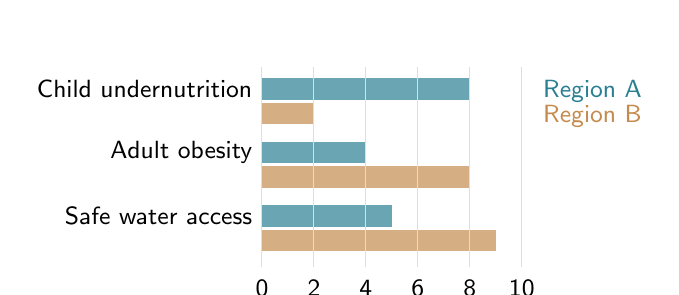
\begin{tikzpicture}[x=0.33cm,y=0.62cm, every node/.style={font=\sffamily\small}]
  \node[anchor=east] at (0,3) {Child undernutrition};
  \draw[fill=AccentTeal!70, draw=none] (0,2.78) rectangle (8,3.22);
  \draw[fill=AccentGold!70, draw=none] (0,2.28) rectangle (2,2.72);
  \node[anchor=east] at (0,1.7) {Adult obesity};
  \draw[fill=AccentTeal!70, draw=none] (0,1.48) rectangle (4,1.92);
  \draw[fill=AccentGold!70, draw=none] (0,0.98) rectangle (8,1.42);
  \node[anchor=east] at (0,0.4) {Safe water access};
  \draw[fill=AccentTeal!70, draw=none] (0,0.18) rectangle (5,0.62);
  \draw[fill=AccentGold!70, draw=none] (0,-0.32) rectangle (9,0.12);
  \foreach \x in {0,2,4,6,8,10} {
    \draw[RuleGray] (\x,-0.65) -- (\x,3.45);
    \node[anchor=north] at (\x,-0.72) {\x};
  }
  \node[anchor=west, color=AccentTeal] at (10.45,2.95) {Region A};
  \node[anchor=west, color=AccentGold] at (10.45,2.45) {Region B};
\end{tikzpicture}
\end{center}

\subsection{Question 1: State Two Contrasts}

\textbf{State two contrasts between Region A and Region B shown in Source A.}
\hfill \textbf{2 points}

\blankbox{white}{3.1cm}

\subsection{Question 2: Describe Indicators}

\textbf{Describe two ways food and health indicators can show inequality.}
\hfill \textbf{4 points}

\blankbox{white}{5.2cm}

\newpage

\subsection{Question 3: Explain Food-System Links}

\textbf{Explain two reasons why food systems can influence health outcomes.}
\hfill \textbf{4 points}

\blankbox{white}{7.4cm}

\subsection{Question 4: Named Example}

\textbf{Using Brazil and Nestle, or the named Food and health case study you
have studied, examine the role of stakeholders in improving or worsening food
security and health.}
\hfill \textbf{10 points}

\blankbox{white}{11.8cm}

\newpage

\section{20-Minute Mark And Error Log}

\subsection{Score Sheet}

\begin{tabularx}{\textwidth}{L{0.16\textwidth}L{0.18\textwidth}Y}
\toprule
\textbf{Question} & \textbf{Score} & \textbf{One reason for the score} \\
\midrule
1 & \rule{0.08\textwidth}{0.4pt} / 2 & \rule{0.58\textwidth}{0.4pt} \\
2 & \rule{0.08\textwidth}{0.4pt} / 4 & \rule{0.58\textwidth}{0.4pt} \\
3 & \rule{0.08\textwidth}{0.4pt} / 4 & \rule{0.58\textwidth}{0.4pt} \\
4 & \rule{0.08\textwidth}{0.4pt} / 10 & \rule{0.58\textwidth}{0.4pt} \\
Total & \rule{0.08\textwidth}{0.4pt} / 20 & \rule{0.58\textwidth}{0.4pt} \\
\bottomrule
\end{tabularx}

\subsection{Error Log}

\rowcolors{2}{TableStripe}{white}
\begin{tabularx}{\textwidth}{L{0.18\textwidth}Y Y Y}
\toprule
\textbf{Error type} & \textbf{What I wrote or missed} & \textbf{Correct version} & \textbf{Next action} \\
\midrule
\rule{0pt}{1.6cm} & & & \\
\rule{0pt}{1.6cm} & & & \\
\rule{0pt}{1.6cm} & & & \\
\rule{0pt}{1.6cm} & & & \\
\bottomrule
\end{tabularx}
\rowcolors{2}{}{}

\subsection{Rewrite One Weak Answer}

Choose the weakest answer and rewrite it below using the correct command term.

\blankbox{SoftTint}{7.1cm}

\newpage

\section{10-Minute Case-Study Drill}

Use this final block only for case-study names and one evaluative point for
each. The keyword table belongs to the recall block.

\begin{tabularx}{\textwidth}{L{0.24\textwidth}Y Y}
\toprule
\textbf{Case-study name} & \textbf{Precise detail} & \textbf{Evaluative point} \\
\midrule
Brazil and Nestle / Nestle Ate Voce & \rule{0.82\linewidth}{0.4pt} & \rule{0.82\linewidth}{0.4pt} \\
Studied disease case, or skip & \rule{0.82\linewidth}{0.4pt} & \rule{0.82\linewidth}{0.4pt} \\
Studied food-security case & \rule{0.82\linewidth}{0.4pt} & \rule{0.82\linewidth}{0.4pt} \\
Future food or health example & \rule{0.82\linewidth}{0.4pt} & \rule{0.82\linewidth}{0.4pt} \\
\bottomrule
\end{tabularx}

\section{Mastery Update}

Rate yourself after marking. Be strict enough that the score is useful.

\begin{tabularx}{\textwidth}{Y L{0.15\textwidth}Y}
\toprule
\textbf{Skill} & \textbf{Rating} & \textbf{Evidence} \\
\midrule
I can recall the Food and health four-cluster map. & \_\_ /5 & \\
I can explain food-system chains using process language. & \_\_ /5 & \\
I can explain disease spread using several factors. & \_\_ /5 & \\
I can use Brazil and Nestle or another named example with evaluation. & \_\_ /5 & \\
I can answer a structured question under time. & \_\_ /5 & \\
\bottomrule
\end{tabularx}

\vspace{0.7em}

\noindent\colorbox{SoftGreen}{%
\begin{minipage}{0.965\textwidth}
\sffamily\raggedright
\textbf{\textcolor{HeadingBlue}{Carry forward to Tuesday 2026-04-28.}}
My weakest Food and health item is:
\rule{0.53\textwidth}{0.4pt}
\end{minipage}
}

\end{document}
